% Sprawozdanie (wersja skrócona): Zadanie 1 -- Korpusy anotowane oraz osadzenia słów i tekstów
% Liczby i tabele z generated/*.tex powstają z plików repo (python report/build_assets.py).
% Word Embeddings: uzupełnij miejsca oznaczone \todo{...}.
\documentclass[11pt,a4paper]{article}

\usepackage[T1]{fontenc}
\usepackage[utf8]{inputenc}
\usepackage{lmodern}
\usepackage[polish]{babel}
\usepackage[margin=2.4cm]{geometry}
\usepackage{microtype}
\usepackage{graphicx}
\usepackage{booktabs}
\usepackage{array}
\usepackage{amsmath}
\usepackage{xcolor}
\usepackage{float}
\usepackage[font=small,labelfont=bf]{caption}
\usepackage{enumitem}
\usepackage[colorlinks=true,linkcolor=blue!50!black,urlcolor=blue!50!black,citecolor=blue!50!black]{hyperref}

\graphicspath{{figures/}}
\setlength{\parindent}{0pt}
\setlength{\parskip}{0.5em}
\setlist{itemsep=0.1em,topsep=0.2em}

\newcommand{\todo}[1]{\par\noindent\fcolorbox{orange!70!black}{yellow!20}{\parbox{\dimexpr\linewidth-2\fboxsep-2\fboxrule\relax}{\small\textbf{DO UZUPEŁNIENIA:} #1}}\par}
\newcommand{\inputorTodo}[2]{\IfFileExists{generated/#1.tex}{\input{generated/#1}}{\todo{#2}}}

\newcommand{\accFasttext}{0{,}505}
\newcommand{\accTfidf}{0{,}490}
\newcommand{\accUse}{0{,}520}
\newcommand{\baseFasttext}{0{,}415}
\newcommand{\baseTfidf}{0{,}415}
\newcommand{\baseUse}{0{,}415}
\newcommand{\corpusConflicts}{6}
\newcommand{\corpusDup}{39}
\newcommand{\corpusFrame}{41\,373}
\newcommand{\corpusLines}{45\,974}
\newcommand{\corpusMean}{17{,}9}
\newcommand{\corpusMedian}{15}
\newcommand{\corpusQhigh}{41}
\newcommand{\corpusQlow}{5}
\newcommand{\corpusUnique}{45\,935}
\newcommand{\finalAmbN}{17}
\newcommand{\foneFasttext}{0{,}322}
\newcommand{\foneTfidf}{0{,}318}
\newcommand{\foneUse}{0{,}330}
\newcommand{\goldAmbKept}{15}
\newcommand{\goldAmbN}{50}
\newcommand{\goldAmbToNeu}{17}
\newcommand{\goldFinalPct}{69{,}5\%}
\newcommand{\goldFinalSame}{139}
\newcommand{\kMarkCohenI}{0{,}463}
\newcommand{\kMarkCohenII}{0{,}420}
\newcommand{\kMarkRawI}{58{,}9\%}
\newcommand{\kMarkRawII}{55{,}8\%}
\newcommand{\kSentCohenI}{0{,}754}
\newcommand{\kSentCohenII}{0{,}710}
\newcommand{\kSentFleissI}{0{,}754}
\newcommand{\kSentFleissII}{0{,}709}
\newcommand{\kSentRawI}{83{,}0\%}
\newcommand{\kSentRawII}{80{,}0\%}
\newcommand{\kTokCohenI}{0{,}730}
\newcommand{\kTokCohenII}{0{,}705}
\newcommand{\kTokRawI}{94{,}4\%}
\newcommand{\kTokRawII}{93{,}8\%}
\newcommand{\nAgreedI}{83}
\newcommand{\nAgreedII}{80}
\newcommand{\nConfI}{17}
\newcommand{\nConfII}{20}
\newcommand{\nMarkI}{231}
\newcommand{\nMarkII}{226}
\newcommand{\nPickAI}{9}
\newcommand{\nPickAII}{10}
\newcommand{\nPickBI}{6}
\newcommand{\nPickBII}{10}
\newcommand{\nPickOtherI}{2}
\newcommand{\nPickOtherII}{0}
\newcommand{\nTokI}{1706}
\newcommand{\nTokII}{1608}
\newcommand{\silFasttext}{$-$0{,}123}
\newcommand{\silTfidf}{$-$0{,}008}
\newcommand{\silUse}{$-$0{,}013}

\IfFileExists{generated/we_macros.tex}{% Generowane przez: python -m src.word_report (nie edytować ręcznie)
\newcommand{\weCosDobrySwietny}{0{,}86}
\newcommand{\weCosDobryZly}{0{,}73}
\newcommand{\weCosPolecamOdradzam}{0{,}79}
\newcommand{\weCovAnnIpi}{94{,}9}
\newcommand{\weCovAnnPol}{83{,}7}
\newcommand{\weCovNegIpi}{91}
\newcommand{\weCovNegPol}{65}
\newcommand{\weCovTokensIpi}{97{,}1}
\newcommand{\weCovTokensPol}{92{,}0}
\newcommand{\weCovTypesIpi}{94{,}6}
\newcommand{\weCovTypesPol}{85{,}2}
\newcommand{\weCtxProbeIpi}{0{,}62}
\newcommand{\weCtxProbePol}{0{,}62}
\newcommand{\weCtxPurityIpi}{0{,}545}
\newcommand{\weCtxPurityPol}{0{,}559}
\newcommand{\weCtxRandIpi}{0{,}502}
\newcommand{\weCtxRandPol}{0{,}504}
\newcommand{\weInVocabIpi}{1423}
\newcommand{\weInVocabPol}{1283}
\newcommand{\weK}{10}
\newcommand{\weNLabelled}{267}
\newcommand{\weNQueries}{215}
\newcommand{\weNSentences}{200}
\newcommand{\weNTokens}{2783}
\newcommand{\weNWords}{1505}
\newcommand{\weOverlap}{9}
\newcommand{\weOverlapShared}{12}
\newcommand{\weOverlapSharedWzm}{18}
\newcommand{\weOverlapWzm}{16}
\newcommand{\wePolOppNegIpi}{17}
\newcommand{\wePolOppNegPol}{20}
\newcommand{\wePolOppPozIpi}{41}
\newcommand{\wePolOppPozPol}{32}
\newcommand{\wePolSameNegIpi}{67}
\newcommand{\wePolSameNegPol}{70}
\newcommand{\wePolSamePozIpi}{47}
\newcommand{\wePolSamePozPol}{59}
\newcommand{\wePolemoSentences}{45\,935}
\newcommand{\wePolemoWords}{679\,251}
\newcommand{\weProbeIpi}{0{,}72}
\newcommand{\weProbePol}{0{,}58}
\newcommand{\weProbeRandIpi}{0{,}50}
\newcommand{\weProbeRandPol}{0{,}50}
\newcommand{\wePurityIpi}{0{,}648}
\newcommand{\wePurityNegIpi}{0{,}47}
\newcommand{\wePurityNegPol}{0{,}37}
\newcommand{\wePurityPol}{0{,}671}
\newcommand{\wePurityPozIpi}{0{,}75}
\newcommand{\wePurityPozPol}{0{,}81}
\newcommand{\wePurityRandIpi}{0{,}536}
\newcommand{\wePurityRandPol}{0{,}571}
\newcommand{\weRhoAll}{0{,}27}
\newcommand{\weRhoWord}{0{,}29}
\newcommand{\weSharedVocab}{20\,206}
\newcommand{\weSilIpi}{0{,}033}
\newcommand{\weSilPol}{0{,}038}
\newcommand{\weStemIpi}{13}
\newcommand{\weStemPol}{2}
\newcommand{\weVocabIpi}{300\,000}
\newcommand{\weVocabPol}{21\,658}
}{}  % Word Embeddings: python -m src.word_report

\title{Zadanie 1: Korpusy anotowane oraz osadzenia słów i tekstów\\[0.3em]
\large PolEmo 2.0 -- anotacja, zgodność anotatorów, osadzenia zdań}
\author{Aleksandra Hendrysiak, Jan Poręba, Bartosz Procki, Igor Sala; Grupa lab. 4 (17:05)}
\date{}

\begin{document}
\maketitle

% -----------------------------------------------------------------------------
\section{Zakres i dane}
Sprawozdanie obejmuje Zadanie 1 część I oraz część II.
Kod i wyniki znajdują się w repozytorium:
\url{https://github.com/JanP2002/NLP_Lab}.

Użyto zdaniowej wersji korpusu PolEmo~2.0 (recenzje hoteli, lekarzy, uczelni i produktów; etykiety
POZ, NEG, NEU, AMB). Po usunięciu \corpusDup{} powtórzeń zostało \corpusUnique{} zdań (średnio \corpusMean{}
tokenów); rozkład etykiet jest niezrównoważony (NEG 36,8\%, POZ 26,7\%, NEU 24,5\%, AMB 12,0\%).
Do anotacji wylosowano dwie rozłączne próbki po 100 zdań (po 25 z każdej klasy etykiety korpusu,
zdania 5--40 tokenów, bez zdań przykładowych z wytycznych); anotatorom pokazano je bez etykiet korpusu.

% -----------------------------------------------------------------------------
\section{Część I: anotacja}

\subsection{Procedura}

Do realizacji zadania, zastosowana została procedura 2+1: dwie osoby (A1, A2) anotowały niezależnie całą próbkę w arkuszach,
a trzecia osoba (superanotator) rozstrzygała zdania, w których ich etykiety się różniły.
Anotacja miała dwa poziomy: \emph{etykieta zdania} (POZ, NEG, NEU, AMB) oraz \emph{etykiety słów}:
wyrażenia nacechowane (WYR\_POZ, WYR\_NEG) i modyfikatory (WZM -- wzmocnienie, OSL -- osłabienie,
ODW -- odwrócenie). Anotatorzy pracowali niezależnie, w osobnej kolejności zdań, według krótkiej
notatki z wytycznymi (wersja~1).

\subsection{Zgodność anotatorów i porównanie iteracji}\label{sec:iter}

Zgodność liczono kappą Cohena i kappą Fleissa (przy dwóch anotatorach niemal identyczne) na poziomie
zdań, wszystkich słów oraz słów zaznaczonych, czyli takich, którym co najmniej jedna osoba nadała etykietę;
Przedziały ufności zostały wyznaczone bootstrapem po zdaniach. Wyniki obu iteracji zestawia tab.~\ref{tab:compare} i
rys.~\ref{fig:compare}.

\begin{table}[H]
\centering\small
\resizebox{\textwidth}{!}{\begin{tabular}{llllrl}
\toprule
Poziom & Miara & Iteracja 1 [CI] & Iteracja 2 [CI] & $\Delta$ & $\Delta$ [95\% CI] \\
\midrule
Zdania & Cohen & 0{,}754 [0{,}64; 0{,}85] & 0{,}710 [0{,}59; 0{,}82] & $-$0{,}044 & [$-$0{,}209; 0{,}121] \\
 & Fleiss & 0{,}754 [0{,}64; 0{,}85] & 0{,}709 [0{,}59; 0{,}82] & $-$0{,}044 & [$-$0{,}210; 0{,}122] \\
\midrule
Tokeny -- wszystkie & Cohen & 0{,}730 [0{,}66; 0{,}80] & 0{,}705 [0{,}62; 0{,}78] & $-$0{,}025 & [$-$0{,}139; 0{,}084] \\
 & Fleiss & 0{,}730 [0{,}66; 0{,}80] & 0{,}705 [0{,}62; 0{,}78] & $-$0{,}025 & [$-$0{,}140; 0{,}084] \\
\midrule
Tokeny -- zaznaczone & Cohen & 0{,}463 [0{,}35; 0{,}57] & 0{,}420 [0{,}30; 0{,}54] & $-$0{,}042 & [$-$0{,}206; 0{,}123] \\
 & Fleiss & 0{,}462 [0{,}34; 0{,}57] & 0{,}414 [0{,}29; 0{,}53] & $-$0{,}048 & [$-$0{,}220; 0{,}121] \\
\bottomrule
\end{tabular}
}
\caption{Zgodność A1--A2 w iteracji~1 (wytyczne v1) i iteracji~2 (wytyczne v2); $\Delta=\kappa_2-\kappa_1$ z 95\% przedziałem ufności różnicy.}
\label{tab:compare}
\end{table}

\begin{figure}[H]
\centering
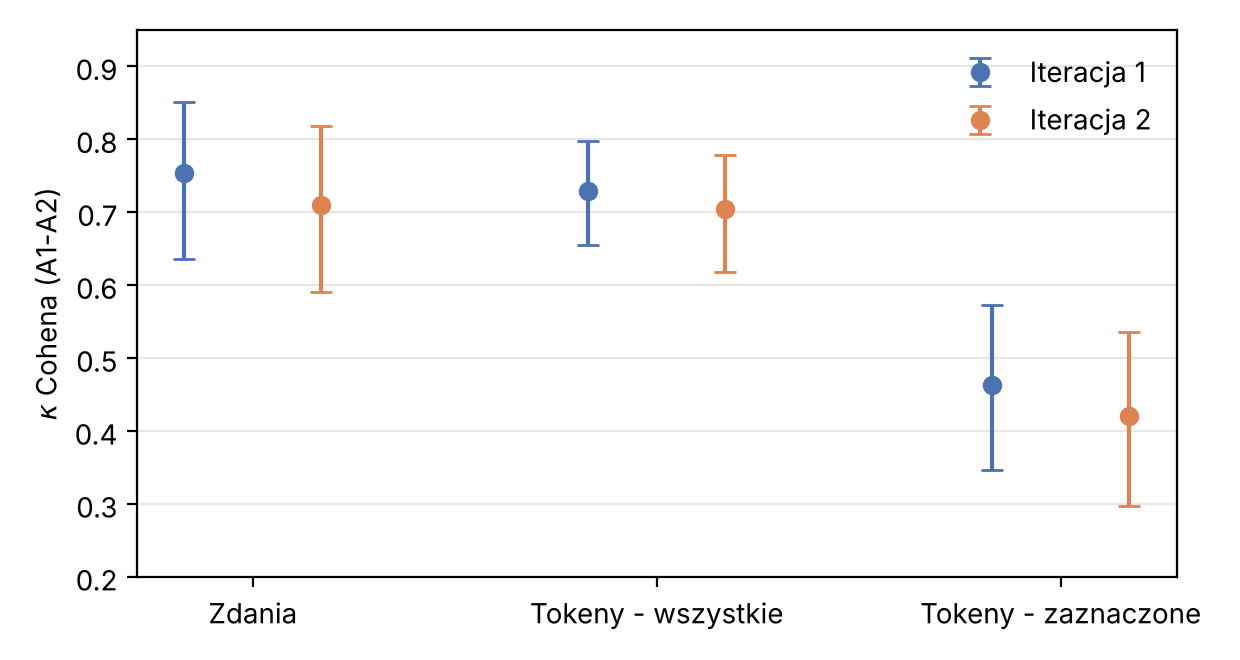
\includegraphics[width=0.66\textwidth]{kappa_comparison.png}
\caption{Kappa Cohena A1--A2 z 95\% przedziałami ufności w obu iteracjach.}
\label{fig:compare}
\end{figure}

W iteracji~1 zgodność na zdaniach wyniosła \kSentRawI{} ($\kappa=\kSentCohenI$, znaczna), na wszystkich słowach
$\kappa=\kTokCohenI$, ale na słowach zaznaczonych tylko $\kappa=\kMarkCohenI$ (umiarkowana): anotatorzy
zgadzali się co do oceny zdania lepiej niż co do tego, \emph{które} słowa ją niosą. Najsłabiej zgodne były
etykiety OSL i WYR\_NEG oraz klasa zdań NEG.

\textbf{Wytyczne v2.} Analiza \nConfI{} rozbieżnych zdań (najczęściej NEG/NEU) wskazała kilka powtarzających
się problemów, na które odpowiedziano w wersji~2: (i) \emph{fakt a opinia} -- sam opis niekorzystnego zdarzenia
bez oceny to NEU; (ii) negatywna ocena jednego aspektu może wystarczyć do NEG; (iii) brak wyraźnej oceny to NEU;
(iv) słowa zależne od kontekstu (\emph{może}, \emph{tylko}, \emph{mało}, \emph{słabo}) nie przesądzają o wydźwięku;
(v) słowa oznacza się według funkcji w zdaniu oraz doprecyzowano AMB, negację i ironię.

\textbf{Wynik iteracji 2.} Zgodność \emph{nie wzrosła}: $\kappa$ na zdaniach spadła z \kSentCohenI{} do
\kSentCohenII{}, na wszystkich słowach z \kTokCohenI{} do \kTokCohenII{}, na słowach zaznaczonych z
\kMarkCohenI{} do \kMarkCohenII{}. Wartości pozostają w tych samych kategoriach, a przedziały ufności różnic
obejmują zero, więc przy 100 zdaniach nie ma podstaw do mówienia o istotnej poprawie ani pogorszeniu.
W podziale na klasy (tab.~\ref{tab:perclass}) zgodność wzrosła dla NEG (z 0,661 do 0,805) i dla fragmentów WYR\_NEG
(0,604 $\to$ 0,698) oraz OSL (0,264 $\to$ 0,468), a spadła dla POZ i AMB (AMB ma tylko 6--10 zdań na osobę, więc ta
wartość jest mało wiarygodna). Konflikty NEG/NEU stały się rzadsze (9 $\to$ 3), zgodnie z intencją reguły o fakcie
i opinii, ale przybyło konfliktów POZ/NEU (4 $\to$ 7) i pojawiły się NEU/AMB (0 $\to$ 3). Może to być spowodowane tym, że nowe reguły przesunęły granicę ku NEU, 
ale kryterium „brak wyraźnej oceny'' bywa nadal rozumiane
różnie; na wynik wpływają też inna próbka i mała liczba zdań.

\begin{table}[H]
\centering\small
\begin{tabular}{lrrrrr}
\toprule
Klasa & $\kappa$ iter.~1 & A1/A2 & $\kappa$ iter.~2 & A1/A2 & $\Delta\kappa$ \\
\midrule
POZ & 0{,}851 & 27/29 & 0{,}703 & 26/23 & $-$0{,}148 \\
NEG & 0{,}661 & 22/24 & 0{,}805 & 23/24 & $+$0{,}144 \\
NEU & 0{,}732 & 42/41 & 0{,}736 & 44/43 & $+$0{,}003 \\
AMB & 0{,}784 & 9/6 & 0{,}423 & 7/10 & $-$0{,}361 \\
\bottomrule
\end{tabular}

\caption{Kappa Cohena dla każdej klasy zdań osobno (klasa kontra reszta); A1/A2 to liczby zdań danej klasy.}
\label{tab:perclass}
\end{table}

\subsection{Rozstrzygnięcie konfliktów i zbiór finalny}

Superanotator rozstrzygnął \nConfI{} (iteracja~1) i \nConfII{} (iteracja~2) rozbieżnych zdań; pozostałe zachowały
wspólną etykietę. Powstał zbiór 200 zdań z uzgodnioną etykietą (\emph{final}): POZ 54, NEG 46, NEU 83, AMB
\finalAmbN{}. Zgodność z etykietą korpusu wynosi \goldFinalPct{} (tab.~\ref{tab:goldfinal}); największa różnica to
zdania z etykietą korpusu AMB, z których \goldAmbToNeu{} z \goldAmbN{} uznano za NEU. Kierunek zmian jest zgodny z
nowymi regułami (brak wyraźnej oceny to NEU); etykieta \emph{final} dotyczy zdania ocenianego bez kontekstu recenzji,
a etykieta korpusu pochodzi z anotacji korpusu, więc różnice nie muszą oznaczać błędu żadnej ze stron.

\begin{table}[H]
\centering\small
\begin{tabular}{lrrrrr}
\toprule
gold $\downarrow$ / final $\rightarrow$ & POZ & NEG & NEU & AMB & razem \\
\midrule
gold POZ & 40 & 0 & 9 & 1 & 50 \\
gold NEG & 1 & 38 & 11 & 0 & 50 \\
gold NEU & 2 & 1 & 46 & 1 & 50 \\
gold AMB & 11 & 7 & 17 & 15 & 50 \\
\midrule
\textbf{razem} & 54 & 46 & 83 & 17 & 200 \\
\bottomrule
\end{tabular}

\caption{Etykieta korpusu (gold) a etykieta uzgodniona (final), 200 zdań.}
\label{tab:goldfinal}
\end{table}

\subsection{Pozostała część zbioru i statystyki opisowe}

Pozostała część zbioru nie została zanotowana. W ramach zadania zanotowano dwie próbki po 100 zdań (łącznie 200 zdań
z uzgodnioną etykietą). Zgodność w iteracji~2 ($\kappa$ Cohena na zdaniach 0,710, znaczna) pozwalałaby przejść do
anotacji reszty zbioru, ale nie została ona wykonana.

Statystyki opisowe uzyskanego zbioru 200 zdań podają tab.~\ref{tab:final} i~\ref{tab:tokcounts}. W obu próbkach
dominuje NEU, a AMB jest rzadkie, przy czym w próbce~2 jeszcze rzadsze (6 zdań wobec 11). Długość zdań jest podobna
(średnio 17,1 i 16,1 tokenów, łącznie 16,6; zakres 5--36). Wśród słów z etykietą przeważają wyrażenia nacechowane
(WYR\_POZ i WYR\_NEG), a modyfikatory są rzadsze; OSL występuje tylko kilka razy na próbkę. Liczby oznaczonych słów
różnią się nieco między anotatorami, co odpowiada umiarkowanej zgodności na słowach zaznaczonych.

\begin{table}[H]
\centering\small
\begin{tabular}{lrrrrrrrr}
\toprule
Iteracja & POZ & NEG & NEU & AMB & razem & śr. tokenów & min & maks \\
\midrule
1 & 27 & 22 & 40 & 11 & 100 & 17,1 & 5 & 36 \\
2 & 27 & 24 & 43 & 6 & 100 & 16,1 & 5 & 35 \\
\midrule
razem & 54 & 46 & 83 & 17 & 200 & 16,6 & 5 & 36 \\
\bottomrule
\end{tabular}
\caption{Zbiór uzgodniony: rozkład etykiet zdań i długość zdań (liczba tokenów) w próbkach.}
\label{tab:final}
\end{table}

\begin{table}[H]
\centering\small
\begin{tabular}{lrrrr}
\toprule
Etykieta słowa & iter.~1: A1 & iter.~1: A2 & iter.~2: A1 & iter.~2: A2 \\
\midrule
WYR\_POZ & 88 & 77 & 95 & 77 \\
WYR\_NEG & 54 & 53 & 56 & 43 \\
WZM & 29 & 31 & 19 & 16 \\
OSL & 9 & 6 & 11 & 6 \\
ODW & 17 & 15 & 20 & 23 \\
\bottomrule
\end{tabular}
\caption{Liczba słów z daną etykietą fragmentu u każdego anotatora (przed rozstrzygnięciem).}
\label{tab:tokcounts}
\end{table}

% -----------------------------------------------------------------------------
\section{Część II: Word Embeddings}\label{sec:we}

W tej części porównano dwa modele word2vec różniące się korpusem uczącym: ogólny model IPI PAN i model wytrenowany
na recenzjach PolEmo. Kod: \texttt{src/word\_embeddings.py} (osadzenia), \texttt{src/word\_tsne.py} (t-SNE),
\texttt{src/word\_neighbours.py} (najbliższe słowa), \texttt{src/word\_report.py} (tabele i liczby do sprawozdania).
\inputorTodo{we_models}{opis modeli i pokrycia słownika}
\inputorTodo{we_tsne}{wykres t-SNE słów}
\inputorTodo{we_knn}{listy najbliższych sąsiadów}
\IfFileExists{sections/we_dyskusja.tex}{% Część II, Word Embeddings, pkt 4: dyskusja (word2vec). Liczby: makra \we... z generated/we_macros.tex
% (python -m src.word_report). Tekst pisany ręcznie -- przy zmianie wyników sprawdzić, czy wnioski nadal się zgadzają.
\subsection{Dyskusja}\label{sec:we-dyskusja}

\textbf{1. Czy osadzenia uczone na dużych korpusach dobrze odwzorowują znaczenie słów w korpusie dziedzinowym?}
Częściowo. Model IPI PAN zna \weCovTypesIpi\% słów i \weCovTokensIpi\% wystąpień naszego korpusu, w tym wszystkie
zaanotowane modyfikatory (tab.~\ref{tab:we-coverage}); braki to głównie słowa rzadkie, formy z cyframi i zapisy bez
polskich znaków. Znaczenie ogólne oddaje trafnie (\emph{lekarz} $\to$ \emph{chirurg, internista}; \emph{brud} $\to$
\emph{smród, kurz}), ale jest to znaczenie słownikowe, a nie to, które słowo ma w recenzji: \emph{miła} ma sąsiadów
\emph{sympatyczna, życzliwa}, a w modelu uczonym na PolEmo \emph{pomocna, uprzejma, profesjonalna} (opinie o lekarzach);
\emph{brudne} ma w nim sąsiadów \emph{wykładziny, kafelki, pleśń} (hotele). Model dziedzinowy płaci za to rozmiarem:
słownik ma tylko \weVocabPol{} słów, a pokrycie spada do \weCovTypesPol\% (\weCovNegPol\% dla słów WYR\_NEG). Oba modele
traktują \emph{ok} (w anotacji ocena pozytywna) jak skrót \emph{około}.

\textbf{2. Czy słowa związane z anotacją grupują się (pozytywne i negatywne)?}
Słabo. Na wykresach t-SNE (rys.~\ref{fig:we-tsne-ipi} i~\ref{fig:we-tsne-pol}) słowa WYR\_POZ i WYR\_NEG są wymieszane.
W przestrzeni 100-wymiarowej słowa o tej samej etykiecie są sobie nieco bliższe niż przy losowym przypisaniu etykiet
(czystość 10 najbliższych sąsiadów \wePurityIpi{} wobec \wePurityRandIpi{}, tab.~\ref{tab:we-separation}), ale nie
tworzą skupisk (sylwetka \weSilIpi{}); bliżej siebie leżą głównie słowa pozytywne (\wePurityPozIpi{}), negatywne nie
(\wePurityNegIpi{}). Antonimy leżą blisko: $\cos(\text{dobry},\text{zły})=\weCosDobryZly$, a \wePolOppPozIpi\% ocenionych
sąsiadów słów pozytywnych ma wydźwięk negatywny (\emph{polecam} $\to$ \emph{odradzam}, \emph{zadowolona} $\to$
\emph{niezadowolona}). Wynika to ze sposobu uczenia: word2vec przewiduje kontekst słowa~\cite{word2vec}, a słowa
o przeciwnym wydźwięku występują w tych samych kontekstach (\emph{obsługa była miła / niemiła}). Wydźwięk zależy też od
dziedziny i negacji; nawet anotatorzy oznaczali \emph{nie} jako odwrócenie tylko w części zdań. Informacja o wydźwięku
nie znika jednak całkiem: prosty klasyfikator odczytuje etykietę WYR\_POZ / WYR\_NEG z wektora IPI PAN z trafnością
\weProbeIpi{} (przy losowych etykietach \weProbeRandIpi{}), choć nie widać jej w sąsiedztwie słów. Wyraźniej słowa
grupują się według funkcji: modyfikatory (\emph{bardzo, bardziej, trochę, całkiem}) tworzą zwarte skupisko.

\textbf{3. Na czym polegają różnice między listami najbliższych słów i z czego wynikają?}
Modele prawie się nie zgadzają: wspólnych jest średnio tylko \weOverlap\% sąsiadów (\weOverlapShared\% przy wyszukiwaniu
we wspólnym słowniku; tab.~\ref{tab:we-knn-overlap}), a korelacja podobieństw między słowami zapytania wynosi
\weRhoAll{}. Różnica nie wynika więc z rozmiaru słowników, lecz z korpusu: model ogólny daje relacje słownikowe
(synonimy, antonimy, wyrazy tej samej kategorii), model z recenzji -- skojarzenia tematyczne
(tab.~\ref{tab:we-knn-examples}). Mały korpus PolEmo (\wePolemoWords{} słów) daje szum dla rzadszych słów
(\emph{problem} $\to$ \emph{kulinarnie, zdrowotny}). Model form IPI PAN częściej zwraca odmiany tego samego słowa
(\weStemIpi\% sąsiadów wobec \weStemPol\%), a zapisy bez polskich znaków tworzą w nim osobne sąsiedztwa (\emph{zaden}
$\to$ \emph{kazdy, zwykly}). Najbardziej zgodne są wzmacniacze (\weOverlapWzm\% wspólnych sąsiadów), których użycie
mało zależy od dziedziny.

\textbf{4. Jak można ulepszyć osadzenia dla tego zadania?}
(1) Dostosować model ogólny do dziedziny: dotrenować go na pełnych recenzjach PolEmo zamiast uczyć mały model od zera.
(2) Dodać wiedzę o wydźwięku: \emph{retrofitting}~\cite{retrofit} z leksykonem (np. emocjonalną Słowosiecią), który
odsuwa od siebie antonimy, albo osadzenia uczone z etykietami zdań PolEmo. (3) Użyć fastText~\cite{fasttext}, którego
n-gramy znakowe radzą sobie z literówkami i zapisem bez polskich znaków. (4) Lematyzować tekst (albo użyć modeli
\emph{lemmas}), aby odmiany nie zajmowały list. (5) Traktować negację jako część jednostki (\emph{nie\_polecam}).
(6) Sięgnąć po modele kontekstowe (np. HerBERT), które rozróżniają znaczenie słowa zależnie od zdania (\emph{ok} jako
ocena i jako skrót).
}{\todo{dyskusja wyników i odpowiedzi na cztery pytania pomocnicze}}

% -----------------------------------------------------------------------------
\section{Część II: Text Embeddings}\label{sec:te}

\subsection{Osadzenia zdań i wizualizacja t-SNE}

Wektory zdań policzone zostały dla 200 zdań z obu próbek, które mają etykiety korpusu, A1, A2 i uzgodnioną.
Użyto dwóch modeli: \textbf{fastText} (model słów dla polskiego z CLARIN-PL, 100 wymiarów; wektor zdania to
średnia wektorów jego słów) oraz \textbf{Universal Sentence Encoder} (wersja wielojęzyczna, 512 wymiarów,
koduje całe zdanie). Jako punkt odniesienia dodany został \textbf{TF-IDF} (widzi tylko wspólne słowa).

Wizualizacje t-SNE (rys.~\ref{fig:tsne-ft}, \ref{fig:tsne-use}). Kolor oznacza etykietę, kształt punktu iterację.

\begin{figure}[H]
\centering
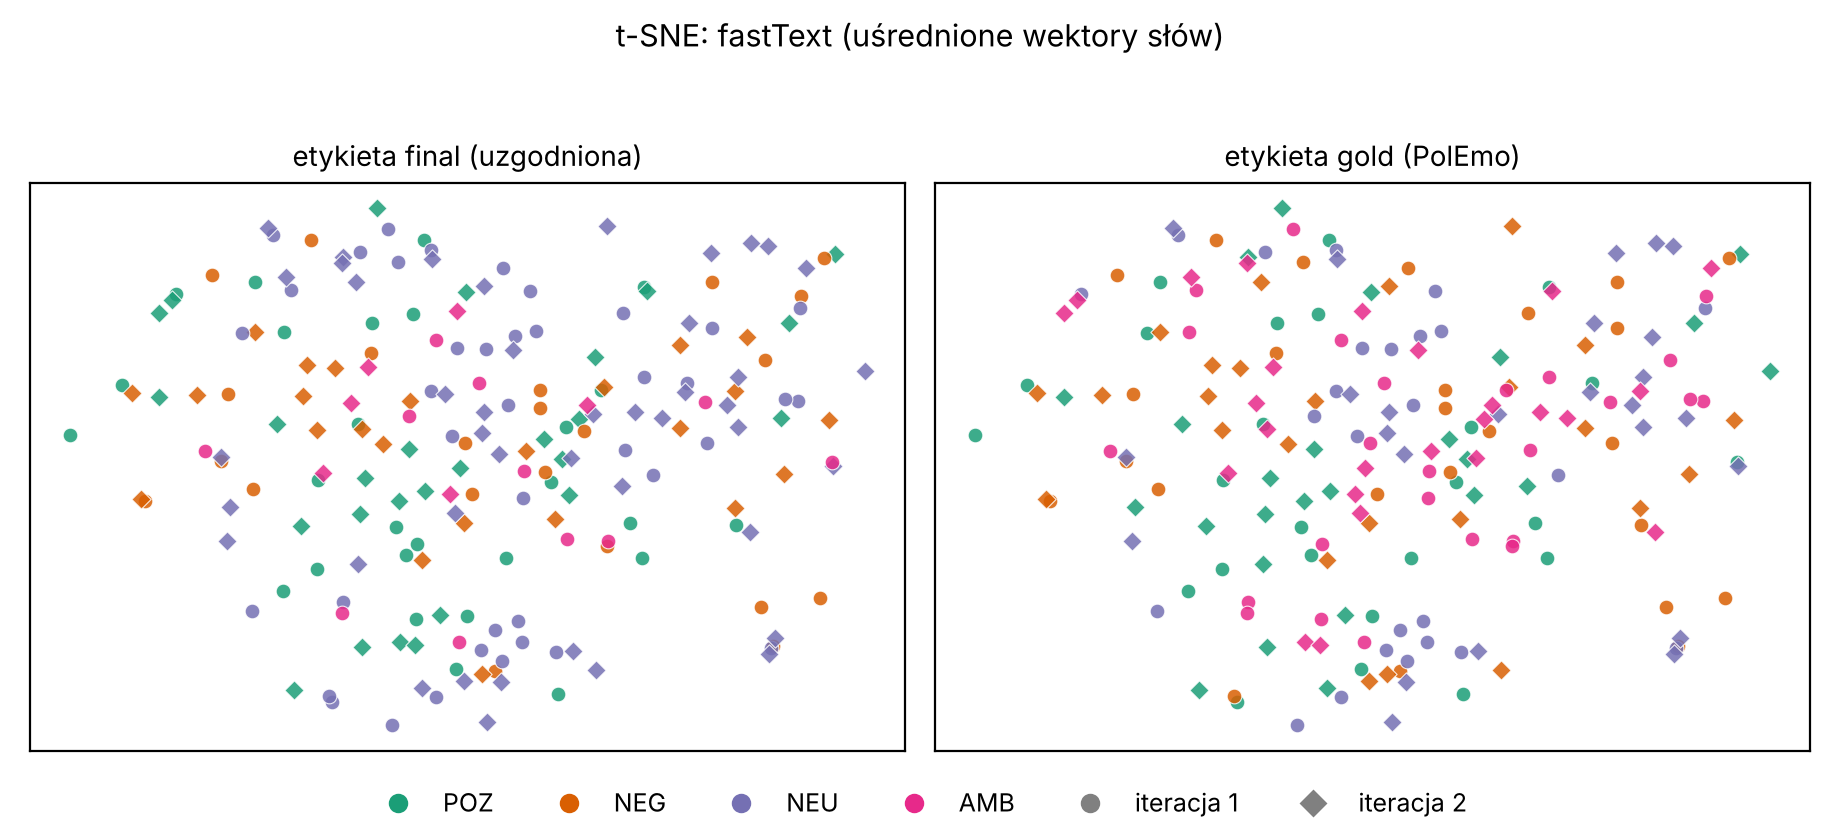
\includegraphics[width=0.95\textwidth]{tsne_fasttext.png}
\caption{t-SNE osadzeń fastText: kolor wg etykiety uzgodnionej (lewy) i korpusu (prawy).}
\label{fig:tsne-ft}
\end{figure}

\begin{figure}[H]
\centering
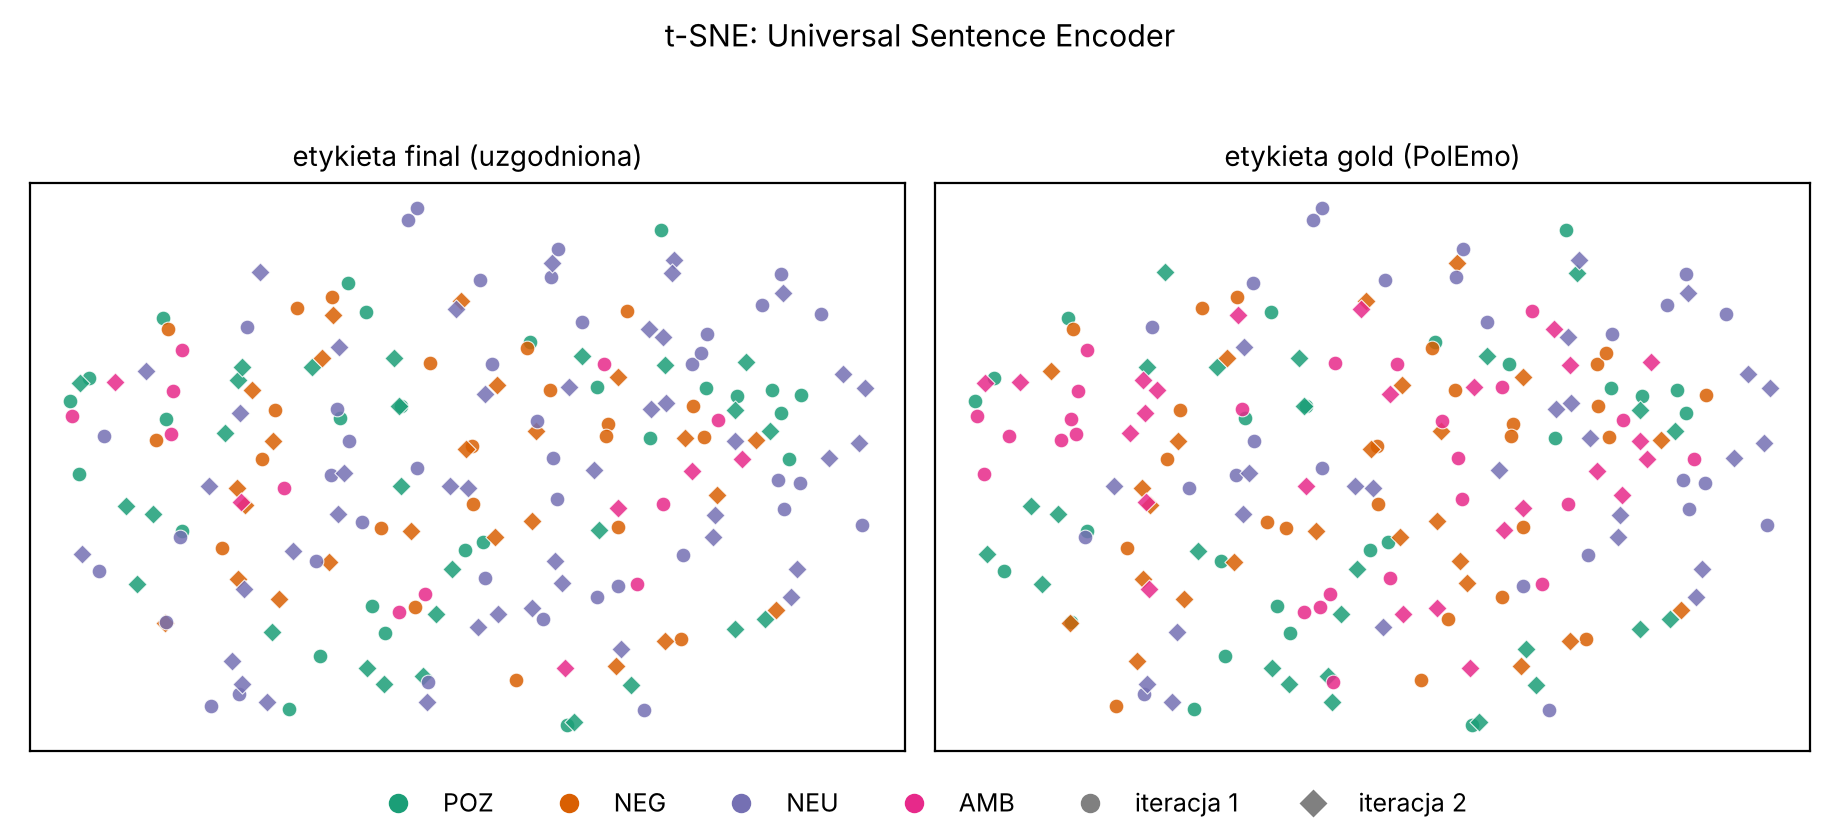
\includegraphics[width=0.95\textwidth]{tsne_use.png}
\caption{t-SNE osadzeń Universal Sentence Encoder.}
\label{fig:tsne-use}
\end{figure}

\textbf{Obserwacje.} W żadnym modelu klasy wydźwięku nie tworzą rozłącznych skupisk: punkty POZ, NEG, NEU i AMB są
w dużej mierze wymieszane, a kolorowanie wg etykiety uzgodnionej i korpusu daje podobny obraz. 
Zgadza się to z miarami ilościowymi (pytanie~5): układ punktów wydaje się odzwierciedlać raczej treść zdań niż ich wydźwięk.

\subsection{Analiza osadzeń i odpowiedzi na pytania}

Odpowiedzi opierają się na ręcznie napisanych parach kontrolnych (parafrazy, przeciwny sens przy podobnych słowach,
ten sam sens w różnej długości, pary niepowiązane; tab.~\ref{tab:probe-means}), na parach zdań z korpusu oraz na
klasyfikatorze wydźwięku uczonym na samych osadzeniach. Przy tak małych zestawach wnioski mają charakter
ilustracji, a nie statystyki.

\begin{table}[H]
\centering\small
\begin{tabular}{lrrr}
\toprule
Kategoria par & fastText & USE & TF-IDF \\
\midrule
parafraza & 0{,}746 & 0{,}492 & 0{,}376 \\
przeciwny sens, podobne słowa & 0{,}859 & 0{,}794 & 0{,}744 \\
przeciwny sens, te same słowa & 0{,}892 & 0{,}924 & 0{,}770 \\
ten sam sens, różna długość & 0{,}604 & 0{,}191 & 0{,}389 \\
kontrola: niepowiązane & 0{,}506 & 0{,}111 & 0{,}004 \\
\bottomrule
\end{tabular}

\caption{Średnie podobieństwo kosinusowe par kontrolnych według kategorii.}
\label{tab:probe-means}
\end{table}

\textbf{1. Czy są zdania uznane za podobne, ale różniące się znaczeniem?} Tak. Pary o przeciwnym sensie i podobnych
słowach mają wyższe podobieństwo niż prawdziwe parafrazy: 0,859 wobec 0,746 w fastText i 0,794 wobec 0,492 w USE;
np.\ „miła''--„niemiła'' daje 0,978 i 0,973. W korpusie najbliższe pary POZ--NEG w fastText (0,90--0,94) dotyczą tego
samego tematu (lekarz, pacjent). W fastText negacja „nie'' ma mały wpływ na średnią wektorów słów, a USE także wyraźnie
nie rozróżnia takich par. Modele kodują więc głównie temat i słownictwo, nie wydźwięk.

\textbf{2. Czy są zdania podobne znaczeniowo, a uznane za odległe, bo użyto innych słów?} Tak. Parafrazy mają niskie
podobieństwo: 0,746 (fastText), 0,492 (USE), 0,376 (TF-IDF); np.\ „Obsługa była bardzo miła i pomocna'' i „Personel okazał
się niezwykle uprzejmy i życzliwy'' dają 0,681, 0,340 i 0,284. TF-IDF zawodzi najbardziej, bo widzi tylko wspólne
słowa. USE ma niskie wartości, ale wyraźnie odróżnia parafrazy od zdań niepowiązanych (0,492 wobec 0,111), natomiast
fastText uznaje za bliskie także zdania niepowiązane (0,506), bo wszystkie zdania są w nim do siebie podobne. W parach
z korpusu USE trafnie zbliżył zdania o czasie („2 miesiące temu'' i „od dwóch miesięcy''), ale pomylił dwie krótkie
oceny o przeciwnym wydźwięku.

\textbf{3. Czy zdania o różnej długości i podobnym sensie są traktowane podobnie?} Nie w pełni. Krótkie zdanie i jego
długa wersja o tym samym sensie mają podobieństwo 0,604 (fastText), 0,191 (USE) i 0,389 (TF-IDF), czyli mniej niż
parafrazy, a w fastText tylko niewiele więcej niż zdania niepowiązane (0,506). Np.\ „Polecam .'' i długa pochwała hotelu
mają 0,662 w fastText i 0,078 w USE. Długie zdanie wnosi dużo dodatkowej treści, a w fastText uśrednianie zbliża je do
przeciętnego wektora korpusu, więc podobne wydaje się niemal do wszystkiego. Zgodny wydźwięk nie wystarcza, by modele
uznały takie zdania za podobne.

\textbf{4. Czy długość zdania wpływa na podobieństwo i „wyrazistość'' wektora?} Tak. W fastText długie zdania (21--36
tokenów) są bliższe średniemu wektorowi korpusu niż krótkie (5--11 tokenów): podobieństwo do środka rośnie z 0,763 do
0,893, a średnie podobieństwo do innych zdań z 0,624 do 0,731 (korelacja rangowa 0,588); jednocześnie maleje długość
wektora (30,3 $\to$ 27,8). Wynika to z uśredniania wektorów słów: w długim zdaniu wkłady się znoszą, a wektor staje się
mniej wyrazisty. W USE efekt jest słabszy (korelacja 0,318). Wysokie podobieństwo w fastText może więc wynikać z samej
długości zdań, a nie z podobnego sensu.

\textbf{5. Czy osadzenia nadają się do anotowanego zadania (wydźwięk zdania)?} Nie. Klasyfikator uczony na samych
osadzeniach (tab.~\ref{tab:classif}) osiąga dla etykiet uzgodnionych accuracy \accFasttext{} (fastText) i \accUse{} (USE)
przy bazie większościowej \baseUse{} (zawsze NEU), czyli przewaga wynosi tylko 0,09--0,10. F1-Macro jest niskie
(\foneFasttext{} i \foneUse{}), silhouette ujemne lub bliskie zeru (\silFasttext{} i \silUse{}), co oznacza brak
skupisk według wydźwięku. Klasyfikator wybiera głównie NEU (rozpoznaje je w 88--92\%), klasę NEG rozpoznaje rzadko
(9--15\%), a AMB wcale (w zbiorze jest tylko 17 takich zdań). Na zbalansowanych etykietach korpusu USE wypada lepiej
niż fastText (macro-F1 0,464 wobec 0,388), ale nadal słabo. Osadzenia mogłyby co najwyżej służyć jako cecha pomocnicza.

\begin{table}[H]
\centering\small
\resizebox{\textwidth}{!}{\begin{tabular}{llrrrrrrr}
\toprule
Model & Etykiety & $n$ & accuracy & baza większ. & macro-F1 & kNN-10 & losowy & silhouette \\
\midrule
fasttext & final & 200 & 0{,}505 & 0{,}415 & 0{,}322 & 0{,}321 & 0{,}305 & $-$0{,}123 \\
 & gold & 200 & 0{,}395 & 0{,}250 & 0{,}388 & 0{,}282 & 0{,}250 & $-$0{,}072 \\
 & A1 & 200 & 0{,}525 & 0{,}430 & 0{,}341 & 0{,}330 & 0{,}312 & $-$0{,}117 \\
 & A2 & 200 & 0{,}495 & 0{,}420 & 0{,}291 & 0{,}304 & 0{,}308 & $-$0{,}147 \\
\midrule
use & final & 200 & 0{,}520 & 0{,}415 & 0{,}330 & 0{,}334 & 0{,}305 & $-$0{,}013 \\
 & gold & 200 & 0{,}465 & 0{,}250 & 0{,}464 & 0{,}321 & 0{,}250 & $-$0{,}003 \\
 & A1 & 200 & 0{,}545 & 0{,}430 & 0{,}342 & 0{,}350 & 0{,}312 & $-$0{,}013 \\
 & A2 & 200 & 0{,}540 & 0{,}420 & 0{,}364 & 0{,}336 & 0{,}308 & $-$0{,}014 \\
\midrule
tfidf & final & 200 & 0{,}490 & 0{,}415 & 0{,}318 & 0{,}335 & 0{,}305 & $-$0{,}008 \\
 & gold & 200 & 0{,}375 & 0{,}250 & 0{,}374 & 0{,}291 & 0{,}250 & $-$0{,}006 \\
 & A1 & 200 & 0{,}485 & 0{,}430 & 0{,}299 & 0{,}356 & 0{,}312 & $-$0{,}008 \\
 & A2 & 200 & 0{,}430 & 0{,}420 & 0{,}266 & 0{,}330 & 0{,}308 & $-$0{,}009 \\
\bottomrule
\end{tabular}
}
\caption{Klasyfikacja wydźwięku zdania na samych osadzeniach (regresja logistyczna, 5-krotna walidacja krzyżowa).
„Baza większ.'' to accuracy klasyfikatora zawsze wybierającego najliczniejszą klasę, „losowy'' to losowanie zgodne
z rozkładem klas (odniesienie dla kNN-10, czyli odsetka sąsiadów tej samej klasy).}
\label{tab:classif}
\end{table}

% -----------------------------------------------------------------------------
\section{Wnioski}

\begin{itemize}
  \item Zgodność anotatorów jest znaczna na poziomie zdań, a umiarkowana dla zaznaczonych słów. Nowe wytyczne nie
        poprawiły jej mierzalnie (różnice mieszczą się w przedziałach ufności); poprawa dotyczy głównie klasy NEG
        oraz słów WYR\_NEG i OSL.
  \item Rozstrzygnięcie konfliktów przesunęło część zdań z etykiet AMB, NEG i POZ korpusu do NEU, zgodnie z regułą
        „fakt a opinia''; zbiór uzgodniony jest niezrównoważony (dominuje NEU, AMB jest rzadkie).
  \item Testowane osadzenia zdań kodują głównie temat i słownictwo, a słabo wydźwięk: zdania o przeciwnym sensie bywają
        bliższe niż parafrazy, a klasyfikator na samych osadzeniach niewiele przewyższa bazę większościową.
  \item Porównując podobieństwa, trzeba uwzględniać długość zdań (uśrednianie zbliża długie zdania do wektora
        średniego) oraz skalę modelu (USE ma niższe wartości niż fastText).
\end{itemize}

\begin{itemize}
  \item Osadzenia word2vec dobrze pokrywają słownictwo korpusu (model IPI PAN zna \weCovTypesIpi\% słów) i oddają
        znaczenie ogólne, ale słabo wydźwięk: antonimy leżą blisko, a słowa pozytywne i negatywne nie tworzą skupisk
        (sylwetka \weSilIpi{}); wydźwięk da się jednak częściowo odczytać prostym klasyfikatorem (trafność \weProbeIpi{}).
  \item Model ogólny i model uczony na recenzjach dają niemal rozłączne listy najbliższych słów (\weOverlap\% wspólnych
        sąsiadów): pierwszy relacje słownikowe (synonimy, antonimy), drugi skojarzenia tematyczne, ale z szumem dla
        rzadkich słów.
  \item Do zadań związanych z wydźwiękiem potrzebna jest adaptacja do dziedziny i wiedza o wydźwięku (np. retrofitting)
        albo modele kontekstowe.
\end{itemize}

\section*{Wykorzystanie narzędzi opartych na modelach językowych}

Anotatorzy A1 i A2 nie korzystali z modeli językowych (zgodnie z wytycznymi).
W pozostałych częściach pracy korzystano z asystenta opartego na modelu językowym (Claude, Anthropic), przy następujących zadaniach:
napisanie kodu i notebooka do osadzeń zdań (fastText, Universal Sentence Encoder, TF-IDF, t-SNE, klasyfikator, miary jakości;
\texttt{src/text\_embeddings.py}, \texttt{notebooks/Text\_Embeddings.ipynb}); przygotowanie placeholderów na odpowiedzi
na pytania pomocnicze do części Text Embeddings oraz szablonu sprawozdania w \LaTeX{} wraz ze skryptem generującym
tabele i rysunki z plików repozytorium.
W części Word Embeddings: napisanie kodu do osadzeń słów, wizualizacji t-SNE, list najbliższych słów i ich porównania
oraz generowania tabel do sprawozdania (\texttt{src/word\_embeddings.py}, \texttt{src/word\_tsne.py},
\texttt{src/word\_neighbours.py}, \texttt{src/word\_report.py}), a także szkicu dyskusji
(\texttt{report/sections/we\_dyskusja.tex}).
Generowane części zostały sprawdzone przez autorów, a ostateczne decyzje zatwierdzili autorzy.

\begin{thebibliography}{99}
\bibitem{cohen} J.~Cohen, \emph{A coefficient of agreement for nominal scales}, Educational and Psychological Measurement 20(1), 1960.
\bibitem{fleiss} J.~L.~Fleiss, \emph{Measuring nominal scale agreement among many raters}, Psychological Bulletin 76(5), 1971.
\bibitem{landis} J.~R.~Landis, G.~G.~Koch, \emph{The measurement of observer agreement for categorical data}, Biometrics 33(1), 1977.
\bibitem{polemo} J.~Kocoń, P.~Miłkowski, M.~Zaśko-Zielińska, \emph{Multi-level sentiment analysis of PolEmo~2.0}, CoNLL 2019.
\bibitem{fasttext} P.~Bojanowski, E.~Grave, A.~Joulin, T.~Mikolov, \emph{Enriching word vectors with subword information}, TACL 5, 2017.
\bibitem{use} D.~Cer et al., \emph{Universal Sentence Encoder}, arXiv:1803.11175, 2018.
\bibitem{word2vec} T.~Mikolov, K.~Chen, G.~Corrado, J.~Dean, \emph{Efficient estimation of word representations in vector space}, arXiv:1301.3781, 2013.
\bibitem{dsmodels} Instytut Podstaw Informatyki PAN, \emph{Modele dystrybucyjne dla języka polskiego (word2vec; pełny NKJP i polska Wikipedia z końca 2016~r.)}, \url{http://dsmodels.nlp.ipipan.waw.pl} (dostęp: 20.10.2026).
\bibitem{retrofit} M.~Faruqui, J.~Dodge, S.~K.~Jauhar, C.~Dyer, E.~Hovy, N.~A.~Smith, \emph{Retrofitting word vectors to semantic lexicons}, NAACL-HLT 2015.
\end{thebibliography}

\end{document}
